
\begin{figure}
	\footnotesize
	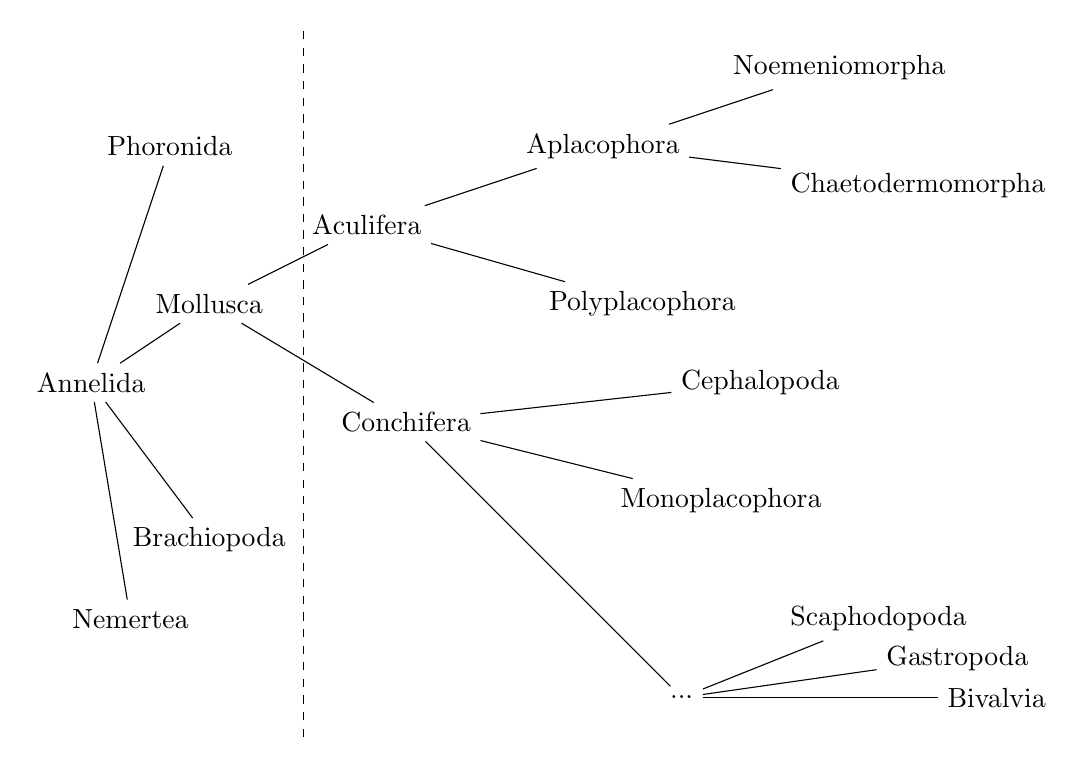
\begin{tikzpicture}
		\node at (1.5,1) (a) {Mollusca};
		\node at (3.5,2) (b) {Aculifera};
		\node at (4,-0.5) (c) {Conchifera};
		\node at (6.5,3) (d) {Aplacophora};
		\node at (7.5,-4) (e) {...};
		\node at (9.5,4) (f) {Noemeniomorpha};
		\node at (10.5,2.5) (g) {Chaetodermomorpha};
		\node at (7,1) (h) {Polyplacophora};
		\node at (8.5,0) (i) {Cephalopoda};
		\node at (8,-1.5)(j) {Monoplacophora};
		\node at (10,-3) (k) {Scaphodopoda};
		\node at (11,-3.5)(l) {Gastropoda};
		\node at (11.5,-4)(m) {Bivalvia};
		\node at (0.5,-3) (n) {Nemertea};
		\node at (1.5,-2) (o) {Brachiopoda};
		\node at (1,3) (p) {Phoronida};
		\node at (0,0) (q) {Annelida};
		
		\draw (q) -- (a);
		\draw (q) -- (n);
		\draw (q) -- (o);
		\draw (q) -- (p);
		
		\draw (a) -- (b);
		\draw (a) -- (c);
		
		\draw (b) -- (d);
		\draw (b) -- (h);
		
		\draw (d) -- (f);
		\draw (d) -- (g);
		
		\draw (c) -- (i);
		\draw (c) -- (j);
		
		\draw (c) -- (e);
		\draw (e) -- (k);
		\draw (e) -- (l);
		\draw (e) -- (m);
		
		\draw[dashed] (2.7,-4.5) -- (2.7,4.5);
	\end{tikzpicture}
	\normalsize
	\caption{Fictitious phylogenesis of Cephalopoda}
	Taxonomic units are ordered by the time of speciation (left to right) and connected by supposed ancestry. (Biological facts were heavily modified by the author.)
	Assuming a query for $v =$ \emph{Chaetodermomorpha} and $s$ represented by the dashed vertical line, \emph{Mollusca} and \emph{Phoronida} are found to be lower and upper bound in the appropriate version of the persistent tree, of which \emph{Mollusca} is found to be ancestor of $v$ through LCA. Finding LCAs of its children and $v$, it is discovered that \emph{Aculifera} is the answer.
	\label{fig:cephalopoda}
\end{figure}